%=====================================================================
%  分片 B：§1.5–§1.10（原文 PDF 第 9–22 页；原文印刷页 8–21）
%  底本：translate/src/src_B.tex；公式、编号、交叉引用逐字照录
%=====================================================================
% （本节重点见 §1 开头，由分片 A 负责）

\subsection{'t Hooft–Polyakov 磁单极}

我们在 Georgi–Glashow 模型中寻找不依赖时间、能量有限的解。能量有限要求：当 $r\rightarrow \infty$ 时，由 (\ref{XXX}) 给出的能量密度 $\theta_{00}$ 必须比 $1/r^3$ 更快地趋于零。这意味着当 $r\rightarrow \infty$ 时，我们的解必须过渡到由 (\ref{XXXI}) 定义的希格斯真空。下面我们先假定这样的有限能量解存在，并证明它可以带有与其孤子数相联系的磁单极荷，而孤子数又由相应的希格斯真空决定。这一结论的证明无需显式处理任何具体解。接下来，我们将介绍 't Hooft–Polyakov 拟设（ansatz），用以具体构造一个这样的磁单极解。我们还会评论双子（dyonic）解的存在性。为方便起见，本节中把矢量记号用于 $SO(3)$ 规范群指标，而不用于空间指标。

% [Tutor Note: 见原文 PDF 第 9 页开头。有限能量条件为 $E=\int\theta_{00}\,d^3x<\infty$：三维体积元带来 $r^2dr$，故要求 $\theta_{00}$ 的衰减快于 $1/r^3$（而不是快于 $1/r^2$）；这里的 $\theta_{00}$ 在静态情形下就是能量密度。]

\noindent\underline{磁荷的拓扑性质：}
\noindent 令 $\vec{\phi}_{vac}$ 表示处于希格斯真空中的场 $\vec{\phi}$。它满足方程
\begin{eqnarray}
&\vec{\phi}_{vac}\cdot\vec{\phi}_{vac} = a^2\,, &\nonumber \\
&\partial_{\mu} \vec{\phi}_{vac}-e\,\vec{W}_{\mu} \times
\vec{\phi}_{vac} = 0\,,& 
\label{vec-vac}
\end{eqnarray}
由此可解出 $\vec{W}_\mu$。最一般的解为
\begin{equation}
\vec{W}_{\mu} = \frac{1}{ea^{2}}\, \vec{\phi}_{vac} \times
\partial_\mu\vec{\phi}_{vac}+\frac{1}{a}\vec{\phi}_{vac}A_{\mu}\,.
\label{sol-vac}
\end{equation}
% [Tutor Note: 见原文 PDF 第 10 页式 (24)。此处系数最容易写错：第一项的 $1/(ea^2)$ 中 $a^2$ 来自 $\vec{\phi}_{vac}\cdot\vec{\phi}_{vac}=a^2$，第二项的 $1/a$ 保证 $A_\mu$ 是归一化的 $U(1)$ 规范场。代回式 (23) 时只需两个恒等式：$\vec{\phi}_{vac}\cdot\partial_\mu\vec{\phi}_{vac}=0$ 与 $(\vec{\phi}_{vac}\times\partial_\mu\vec{\phi}_{vac})\times\vec{\phi}_{vac}=a^2\partial_\mu\vec{\phi}_{vac}$。]
为看出它确实满足 (\ref{vec-vac})，注意 $\partial_\mu\vec{\phi}_{vac}\cdot\vec{\phi}_{vac}=0$，于是
$$
\frac{1}{ea^2}(\vec{\phi}_{vac}\times\partial_{\mu}\vec{\phi}_{vac})
\times \vec{\phi}_{vac}= \frac{1}{ea^2}\left(\partial_\mu\vec{\phi}_{vac}a^2
-\vec{\phi}_{vac} (\vec{\phi}_{vac}\cdot\partial_\mu\phi_{vac})\right)= 
\frac{1}{e}\partial_\mu\vec{\phi}_{vac}\,.
$$
式 (\ref{sol-vac}) 右端第一项是特解，而 $\vec{\phi}_{vac}A_\mu$ 是齐次方程的通解。利用这个解，我们现在可以计算场强张量 $\vec{G}_{\mu\nu}$。对应于规范群未破缺部分的场强 $F_{\mu\nu}$ 可确定为
\begin{eqnarray}
F_{\mu\nu}&=&\frac{1}{a}\vec{\phi}_{vac}\cdot\vec{G}_{\mu \nu}
\nonumber\\
&=&\partial_\mu A_\nu -\partial_\nu A_\mu +
\frac{1}{a^3 e}\vec{\phi}_{vac}\cdot (\partial_\mu\vec{\phi}_{vac}
\times\partial_\nu\vec{\phi}_{vac})\,.
\label{F-vac}
\end{eqnarray}
利用希格斯真空中的运动方程可得
$$
\partial_\mu F^{\mu\nu}=0\,,\qquad \partial_\mu\,\widetilde F^{\mu\nu}=0\,.
$$
这证实 $F_{\mu\nu}$ 是一个合法的 $U(1)$ 场强张量。磁场由 $B^i=-\frac{1}{2}\epsilon^{ijk}F_{jk}$ 给出。现在考虑一个静态、能量有限的解，以及一个包围该解核心的曲面 $\Sigma$。我们取 $\Sigma$ 足够远，使其上解已处于希格斯真空中。于是可以用希格斯真空中的磁场来计算与该解相联系的磁荷 $g_\Sigma$：
\begin{equation}
g_\Sigma=\int_\Sigma\,B^i ds^i=-\frac{1}{2 ea^3} \int_\Sigma\, 
\epsilon_{ijk}\,\vec{\phi}_{vac}\cdot \left(\partial^j\vec{\phi}_{vac}
\times\partial^k\vec{\phi}_{vac}\right)ds^i\,.
\label{XL}
\end{equation}
下面说明右端的表达式是一个拓扑量：由于 $\phi^2=a$，希格斯真空的流形（${\cal M}_0$）具有 $S^2$ 的拓扑。
% [Tutor Note: 原文笔误，见原文 PDF 第 10 页式 (26) 之后。“Since $\phi^2=a$;”有两处问题：(1) 应为 $\phi^2=a^2$，与式 (23) 一致；(2) 分号应为逗号。译文照录公式原样，只按文意断句。]
场 $\vec{\phi}_{vac}$ 定义了从 $\Sigma$ 到 ${\cal M}_0$ 的映射。由于 $\Sigma$ 也是 $S^2$，映射 $\phi_{vac}:\Sigma\rightarrow{\cal M}_0$ 由其同伦群 $\pi_2 (S^2)$ 刻画。换言之，$\phi_{vac}$ 由一个整数 $\nu$（绕数）刻画，它计算该映射把 $\Sigma$ 缠绕到 ${\cal M}_0$ 上的次数。用映射 $\phi_{vac}$ 表示，这个整数为
\begin{equation}
\nu = \frac{1}{4\pi a^{3}} \, \int_\Sigma\,\frac{1}{2}
\epsilon_{ijk}\vec{\phi}_{vac}\cdot\left(\partial^j\vec{\phi}_{vac}
\times \partial^k\vec{\phi}_{vac}\right)\,d s^i\,.
\label{XLI}
\end{equation}
与磁荷的表达式比较，我们得到重要结果
\begin{equation}
g_{\Sigma} = - \frac{4\pi \nu}{e}\,.
\label{XLII}
\end{equation}
% [Tutor Note: 见原文 PDF 第 10 页式 (28)。原文说它与狄拉克条件“相差因子 2”，核对如下：取 $q_0=e\hbar/2$，则 $g_\Sigma q_0/(4\pi\hbar)=-\nu/2$，而狄拉克条件为 $qg/(4\pi\hbar)=n/2$，故要求 $\nu=-n$。式 (26) 中的负号来自 $B^i=-\frac{1}{2}\epsilon^{ijk}F_{jk}$ 与曲面定向的约定，不要与式 (27) 中 $\nu$ 的符号约定混为一谈。]
因此，孤子的绕数决定它的磁单极荷。注意上式与狄拉克量子化条件相差一个因子 $2$。这是因为本模型中可能存在的最小电荷是 $q_0=e\hbar/2$，用它可把 (\ref{XLII}) 化为狄拉克条件。

\noindent\underline{磁单极的拟设：}
\noindent 现在我们介绍 't Hooft \cite{thooft} 与 Polyakov \cite{polya} 提出的拟设，用于在 Georgi–Glashow 模型中构造磁单极解。对于球对称、宇称不变、静态且能量有限的解，他们提出：
\begin{eqnarray}
\phi^a & = & \frac{x^a}{er^2}\,H(aer)\,,\nonumber\\
W^a_i&=&-\epsilon^a_{ij}\frac{x^j}{er^2}\left(1 - K(aer)\right)\,,
\qquad W^a_0= 0\,.
\label{tp-ansatz}
\end{eqnarray}
对于 $r\rightarrow\infty$ 处的非平凡希格斯真空，他们取 $\phi^c_{vac}=ax^c/r= a\hat{x}^c$。注意这把空间无穷远处的 $S^2$ 映到真空流形上，绕数为 1。函数 $H(aer)$ 与 $K(aer)$ 的渐近行为由 $r\rightarrow\infty$ 时的希格斯真空以及 $r=0$ 处的正则性决定。具体地，定义 $\xi=aer$，我们有：当 $\xi\rightarrow\infty,\,H\sim\xi,\, K\rightarrow 0$，当 $\xi\rightarrow 0,\, H\sim\xi,\,(K-1)\sim\xi$。该解的质量可参数化为
$$
M = \frac{4 \pi a}{e} f \, (\lambda /e^{2})
$$
% [Tutor Note: 见原文 PDF 第 11 页式 (29) 之后。核对边界条件：$r\to0$ 时 $H\sim\xi$ 使 $\phi^a=(x^a/er^2)H\to c_1x^a\to0$，故场在原点正则；$r\to\infty$ 时 $H\sim\xi$ 给出 $\phi^a\to ax^a/r=a\hat{x}^a$，而 $K\to0$ 给出 $W^a_i\to-\epsilon^a_{ij}x^j/er^2$。注意 $H$、$K$ 的自变量是 $\xi=aer$ 而不是 $r$，做量纲核对时不要丢掉 $e$ 与 $a$。]
对该拟设，运动方程约化为关于 $K$ 与 $H$ 的两个耦合方程，它们只在某些极限下才能精确求解。当 $r\rightarrow 0$ 时，得到 $H\rightarrow ec_1 r^2$ 与 $K=1+ec_2r^2$，这表明场在 $r=0$ 处不奇异。当 $r\rightarrow\infty$ 时，我们得到 $H\rightarrow\xi+c_3 exp(-a\sqrt{2\lambda}r)$ 与 $K\rightarrow c_4\xi exp(-\xi)$，从而 $W^a_i\approx-\epsilon^a_{ij}x^j/er^2$。再次定义 $F_{ij}=\phi^c G^c_{ij}/a$，磁场为 $B^{i} = - x^i/e r^3$。相应的磁单极荷为 $g=-4\pi/e$，这与该解的绕数为 1 所预期的一致。应当指出，'t Hooft 对阿贝尔场强张量的定义略有不同，但在大距离下它化为上述形式。

注意在上述磁单极解中，狄拉克弦的出现并不显然。为了把狄拉克弦提取出来，我们必须对该解作一个奇异规范变换，把非平凡的希格斯真空 $\phi^c_{vac}=a\hat{x}^c$ 旋转为平庸真空 $\phi^c_{vac}= a \delta^{c3}$。在此过程中，规范场产生了狄拉克弦奇点，它现在充当磁荷的源 \cite{thooft}。

\noindent\underline{Julia–Zee 双子：}

't Hooft–Polyakov 磁单极携带一个单位的磁荷，不带电荷。Georgi–Glashow 模型也允许既带磁荷又带电荷的解。构造这类解的一个拟设由 Julia 与 Zee \cite{Julia-Zee} 提出。在该拟设中，$\phi^a$ 与 $W^a_i$ 的形式与 't Hooft–Polyakov 拟设完全相同，但 $W^a_0$ 不再为零：$W^a_0=x^a J(aer)/er^2$。它充当双子电荷的源。双子的电荷依赖于一个连续参数，在经典层次上并不满足量子化条件。然而，半经典论证 \cite{TW1,GSW} 表明，在 CP 不变的理论中，在量子层次上，双子的电荷量子化为 $q=n\hbar e$。只要认识到磁单极在规范变换下并非不变（而规范变换当然是运动方程的对称性），这一点就很容易理解。为正确处理相应的零模，应把规范自由度视为集体坐标。经过量子化，这个集体坐标导致磁单极存在带离散电荷的带电态。当拉格朗日量中存在破坏 CP 的项时，情况更为微妙，我们将在后面讨论。在下一小节中，我们将描述一个极限，在其中 't Hooft–Polyakov 与 Julia–Zee 拟设的运动方程可以精确求解。这就是孤子质量达到 Bogomol'nyi 界饱和的极限。
% [Tutor Note: 原文 PDF 第 11 页这一段有数处拼写笔误：“easiy”应为“easily”，“guage”应为“gauge”，“treate”应为“treat”，“depends of”应为“depends on”；译文均按原意处理。关于集体坐标论证：静态双子解带有一个连续参数（即 $W^a_0$ 的系数），它对应于保持希格斯真空的 $U(1)$ 规范方向的零模；把该规范自由度作为集体坐标量子化后，其共轭动量（电荷）取分立值 $q=n\hbar e$，细节见文献 [12,13]。]

\subsection{Bogomol'nyi 界与 BPS 态}

本小节中，我们导出双子质量上的 Bogomol'nyi 界 \cite{bogomol}，用其电荷与磁荷（它们是 $F^{\mu\nu}=\vec{\phi}\cdot \vec{G}^{\mu\nu}/a$ 的源）来表示。利用比安基恒等式 (\ref{bianchi}) 以及 (\ref{XXIX}) 中的第一个方程，可把这些荷写成
\begin{eqnarray} 
g&\equiv&\int_{S^2_\infty}B_i dS^i=\frac{1}{a}\int{\cal B}^a_i\phi^a
dS^i = \frac{1}{a} \int {\cal B}^a_i (D^i \phi)^a d^3x\,,
\nonumber\\
q&\equiv&\int_{S^2_\infty}E_i dS^i=\frac{1}{a}\int{\cal E}^a_i\phi^a
dS^i = \frac{1}{a} \int {\cal E}^a_i (D^i \phi)^a d^3x\,. 
\label{gq}
\end{eqnarray}
% [Tutor Note: 见原文 PDF 第 12 页式 (30)。把面积分化为体积分用了两个不同方程：磁荷用非阿贝尔比安基恒等式 $D_i{\cal B}^a_i=0$，电荷用高斯定律（即 (\ref{XXIX}) 的第一个方程）。注意等号链中“面积分”与“体积分”之间的那一步并不只是把 $a$ 提出：需要把 $\phi^a/a$ 作为单位矢量场、分部积分并用 $D_i{\cal B}^a_i=0$，才能把被积函数中的 $\phi^a$ 换成 $(D^i\phi)^a$；这是本节最容易被读者一带而过的地方。]
现在，在质心系中，双子的质量由下式给出
$$
M\equiv \int d^3x \theta_{00}= \int d^3x \left(\,\frac{1}{2}
\left[({\cal E}^a_k)^2+({\cal B}^a_k)^2 + (D_k\phi^a)^2 + 
(D_0\phi^a)^2 \right]+ V(\phi) \right)\,,
$$
其中 $\theta_{\mu\nu}$ 是能量动量张量。稍加运算，并利用 (\ref{gq}) 中给出的电荷与磁荷表达式，可把它写成
\begin{eqnarray}
M&=&\int d^3x \left(\,\frac{1}{2}\left[({\cal E}^a_k -
D_k\phi^a\sin\theta)^2 + ({\cal B}^a_k-D_k\phi^a\cos\theta )^2
+(D_0\phi^a)^2\right] + V(\phi) \right)
\nonumber\\
&+& a (q \sin \theta + g \cos \theta )\,,
\label{M-bog}
\end{eqnarray}
% [Tutor Note: 易错预警，见原文 PDF 第 12 页式 (31)。平方配方时务必与式 (30) 中 $g,q$ 的定义对照：把方括号内展开，除保留 $\frac12[({\cal E}^a_k)^2+({\cal B}^a_k)^2+(D_k\phi^a)^2+(D_0\phi^a)^2]$ 外，交叉项为 $-\sin\theta\,{\cal E}\cdot D\phi-\cos\theta\,{\cal B}\cdot D\phi=-a(q\sin\theta+g\cos\theta)$（注意是负号！），移项后才得到式 (31) 末行的 $+a(q\sin\theta+g\cos\theta)$。若把交叉项符号弄反，就会得出 $M\le a\sqrt{q^2+g^2}$ 的错误结论。对 $\theta$ 求极值时用 $\tan\theta=q/g$，最大值为 $\sqrt{q^2+g^2}$。]
其中 $\theta$ 是任意角。由于第一行中的各项为正，我们可以写出 $M\geq (q \sin \theta + g \cos \theta )$。该界在 $\tan\theta = q/g$ 时取最大。于是得到双子质量上的 Bogomol'nyi 界
$$
M \geq a\, \sqrt{g^2 + q^2}\,.
$$
对 't Hooft–Polyakov 解，我们有 $q = 0$，因此 $M \geq a|g|$。但 $|g|=4\pi/e$，且 $M_W=ae\hbar=aq$，所以
$$
M \geq a \frac{4 \pi}{e} = \frac{4 \pi}{e^{2}\hbar} M_{W} =
\frac{4 \pi \hbar}{q^{2}} M_{W} = \frac{\nu}{\alpha} M_{W}\,.
$$
这里 $\alpha$ 是精细结构常数，$\nu=1$ 或 $1/4$，取决于电子电荷取 $q$ 还是 $q/2$。由于 $\alpha$ 是一个很小的数（对电磁相互作用 $\sim 1/137$），上述关系意味着磁单极远比与对称性破缺相联系的 W 玻色子重。
% [Tutor Note: 见原文 PDF 第 12 页。此处对 $\hbar$ 的处理较随意：由 $M_W=ae\hbar=aq$ 与 $\nu/\alpha$ 的写法可反推出 $\alpha\equiv q^2/(4\pi\hbar)$，只有取 $\hbar=1$ 时才与通常的 $\alpha=e^2/4\pi\sim1/137$ 相符。原文此处只作定性结论（磁单极远重于 W 玻色子），不必纠结 $\hbar$ 的幂次；$\nu=1$ 或 $1/4$ 则取决于把“电子电荷”取作 $q$ 还是 $q/2$。]
由 (\ref{M-bog}) 可见，除非 $\lambda\rightarrow 0$ 使 $V(\phi)=0$，否则界不会饱和。这就是理论的 Bogomol'nyi–Prasad–Sommerfield（BPS）极限 \cite{bogomol,PS}。注意在此极限下，$\phi_{vac}^2 =a^2$ 不再由理论决定，因此必须作为希格斯场的边界条件加上。此外，在此极限下希格斯标量变为无质量。现在，为使界饱和，我们必须取
\begin{equation}
D_0 \phi^a=0\,,\qquad {\cal E}^a_k=(D_k\phi)^a\sin\theta\,,
\qquad{\cal B}^a_k = (D_k\phi)^a\cos\theta\,,
\label{L}
\end{equation}
其中 $\tan\theta=q/g$。在 BPS 极限下，可以在 (\ref{XXIX}) 中或在 (\ref{L}) 中使用 't Hooft–Polyakov（或 Julia–Zee）拟设，从而得到精确的磁单极（或双子）解 \cite{bogomol, PS}。这些解自动达到 Bogomol'nyi 界，被称为 BPS 态。还要注意，在 BPS 极限下，理论的所有微扰激发都达到该界，因而属于 BPS 谱。我们将在后面看到，在 $N=2$ 超对称理论中 BPS 界以非常自然的方式出现。
% [Tutor Note: 见原文 PDF 第 13 页。式 (32) 其实是两类一阶（BPS）方程的合写：$D_0\phi=0$ 与 $\vec{\cal E}=\sin\theta\,D\phi$、$\vec{\cal B}=\cos\theta\,D\phi$；把 't Hooft–Polyakov 拟设代入这些一阶方程即可精确求解（原文引 [14,15]）。另注意：$\lambda\to0$ 时 $V=0$，$a$ 不再由势的极小值固定，故 $|\phi|=a$ 只能作为边界条件强加，这一点在后文 Seiberg–Witten 分析中至关重要。]

\subsection{远距离下的磁单极}

迄今为止，我们都是从理论的希格斯真空结构出发来描述 Georgi–Glashow 模型中产生的磁单极。本节将考虑一般杨–米尔斯–希格斯系统中的磁单极，并把希格斯真空的描述与用未破缺规范场给出的描述联系起来。这些规范场保持无质量，是研究大距离下磁单极时相关的场。这种表述便于描述非阿贝尔磁单极。

设 $\phi$ 按规范群 $G$ 的某个给定表示中的矢量变换。为记号方便，下文我们不再区分群元素 $g$ 与它的某一具体实现。把规范场写成 $W_\mu=T^aW^a_\mu$，我们可以构造 $\phi$ 的协变导数与 $W_\mu$ 的曲率张量如下
\begin{eqnarray}
D_\mu \phi &=& \partial_{\mu} \phi + ie W_{\mu} \phi\,,
\nonumber \\
G_{\mu\nu}&=&\partial_\mu W_\nu -\partial_\nu W_\mu +
ie [W_\mu, W_\nu] \,.
\nonumber
\end{eqnarray}
% [Tutor Note: 术语与记号说明，见原文 PDF 第 13 页。原文用同一个字母 $g$ 表示两件完全不同的东西：群元素 $g$（如式 (36) 的 $g(s,t)$）与磁荷 $g$（见式 (30) 与式 (35)）。阅读时须按上下文区分，切勿把 $g(s,t)$ 的指标结构套到磁荷上。]
拉格朗日密度 ${\cal L}$、能量动量张量 $\theta_{\mu\nu}$ 与规范流 $j^a_\mu$ 则如下给出
\begin{eqnarray}
{\cal L}&=&-\frac{1}{4}(G^a_{\mu\nu})^2+(D^\mu\phi)^\dagger D_\mu\phi
-V(\phi) \,,
\nonumber\\
\theta_{\mu\nu}&=&-G^a_{\mu\lambda}G^{a\lambda}_\nu +
(D_\mu\phi)^\dagger(D_\nu\phi) + (D_\nu\phi)^\dagger(D_\mu\phi) 
- g_{\mu\nu} {\cal L} \,,
\nonumber \\
\theta_{00}&=& \frac{1}{2}{\cal E}^{ia}{\cal E}^a_i +
\frac{1}{2}{\cal B}^{ia}{\cal B}^a_i +D_0\phi^\dagger D_0\phi +
D_i\phi^\dagger D_i\phi + V(\phi)\,,
\nonumber \\
j^a_\mu &=& ie \phi^\dagger T^a D_\mu\phi -
ie (D_\mu\phi)^\dagger T^a \phi\,.
\label{LIII}
\end{eqnarray}
这里希格斯势是规范不变的：$V(g\phi)=V(\phi)$。由上述拉格朗日量得到的运动方程为
\begin{equation}
D^\mu D_\mu\phi^a=-\frac{\partial V}{\partial \phi^a}\,,\qquad
D^\nu G^a_{\mu\nu} = - j_\mu^a\,.
\label{LIV}
\end{equation}
当规范群 $SO(3)$ 自发破缺到 $U(1)$ 时，我们可以像上一节那样精确算出 Bogomol'nyi 界，结果为
\begin{equation}
M\geq \sqrt 2 \, a \sqrt{g^2 + q^2}\,.
\label{Bbound}
\end{equation}
% [Tutor Note: 易错预警，见原文 PDF 第 14 页式 (35)。与 §1.6 的 $M\ge a\sqrt{g^2+q^2}$ 相比这里多出因子 $\sqrt2$：式 (33) 的希格斯动能是复标量的 $(D_\mu\phi)^\dagger D^\mu\phi$，平方配方时须写成 $\frac{1}{2}|{\cal E}-\sqrt2\,D\phi\sin\theta|^2$、$\frac{1}{2}|{\cal B}-\sqrt2\,D\phi\cos\theta|^2$ 之类的形式（实部、虚部各贡献一份），交叉项才给出 $\sqrt2\,a(q\sin\theta+g\cos\theta)$；若照搬 §1.6 实伴随场的 $\frac12(D\phi)^2$ 配方，就会漏掉这个 $\sqrt2$。]
对一般的规范群 $G$，如 Georgi–Glashow 模型那样，希格斯真空由下式定义
$$
V(\phi)=0\,,\qquad D_\mu\phi=0 \,.
$$
第一个方程定义了真空流形 ${\cal M}_0\equiv \{\phi\,: V(\phi)=0\}$，第二个方程给出
$$
[D_\mu, D_\nu] \phi =G_{\mu\nu} \phi = 0\,. 
$$
因此，在希格斯真空中，$G_{\mu\nu}$ 取值于规范群 $G$ 中保持希格斯真空不变的某个子群。我们用 $H$ 表示 $G$ 的这个未破缺子群。$G$ 中不保持希格斯真空不变的生成元当然被破缺，相应的规范玻色子获得质量。如果 $V(\phi)$ 没有额外的整体对称性与偶然的极小值，那么可以合理地假定 $G$ 在 ${\cal M}_0$ 上的作用是传递的。这意味着 ${\cal M}_0$ 中任一点都可通过 $G$ 的某个元素与任意另一点（特别是与某个参考点 $\phi_0$）相联系。因此，${\cal M}_0$ 中任一点的小群（不变群）$H\subset G$ 都同构于其他任一点的小群。于是 ${\cal M}_0$ 的结构由右陪集 $G/H$ 描述。
% [Tutor Note: 含糊点拨，见原文 PDF 第 14 页。原文“$G_{\mu\nu}$ 取值于 $G$ 的某个子群”严格说应为“取值于该子群的李代数”；这里只是省略了“李代数”三字，物理内容不变。又：原文此处有重复词 “the the little group”，系笔误。]
为使解具有有限能量，在离解核心足够远处，场 $\phi$ 必须取值于希格斯真空中。设 $\Sigma$ 是包围核心的一个二维曲面，使得在它上面 $\phi$ 已处于 ${\cal M}_0$ 中。在此曲面上，$\phi$ 描述一个从 $\Sigma$（具有 $S^2$ 的拓扑）到 ${\cal M}_0$ 的映射。该映射由其同伦类刻画，同伦类必须是 $\pi_2({\cal M}_0)\simeq \pi_2(G/H)$ 的一个元素。如前所述，相应的拓扑数就是解的磁荷。只要没有磁单极穿过曲面 $\Sigma$，$\phi$ 就保持为时间的连续函数，其同伦类不变。要证明映射 $\phi$ 满足 $\pi_2(G/H)$ 的群性质，必须考虑若干彼此远离的磁单极，并研究它们的磁荷如何合成。关于这一问题的讨论见 \cite{coleman1}。

以上关于磁单极拓扑刻画的讨论是基于希格斯真空的结构。然而，用未破缺规范场来描述更为自然。这两种描述之间的关系包含在方程 $D_\mu\phi =0$ 之中，该方程在 $S^2$ 曲面 $\Sigma$ 上成立。让我们用正方形 $\{ 0 \leq s, t \leq 1 \}$ 来参数化 $S^2$。从这个正方形到球面的映射 $r(s,t)$ 除在正方形的边界上外处处单值，而该边界被等同于球面上的一个点：
% [Tutor Note: 原文笔误，见原文 PDF 第 14 页：“from this square to the sphare” 中 “sphare” 应为 “sphere”。]
$$
r(0,t) = r(1,t) =r(s,0) =r(s,1) = r_0\,.
$$
固定 $s$ 时，当 $t$ 从 $0$ 变到 $1$，$r(s,t)$ 描述 $S^2$ 上的一条闭路径。

\begin{figure}[htbp]
  \centering
  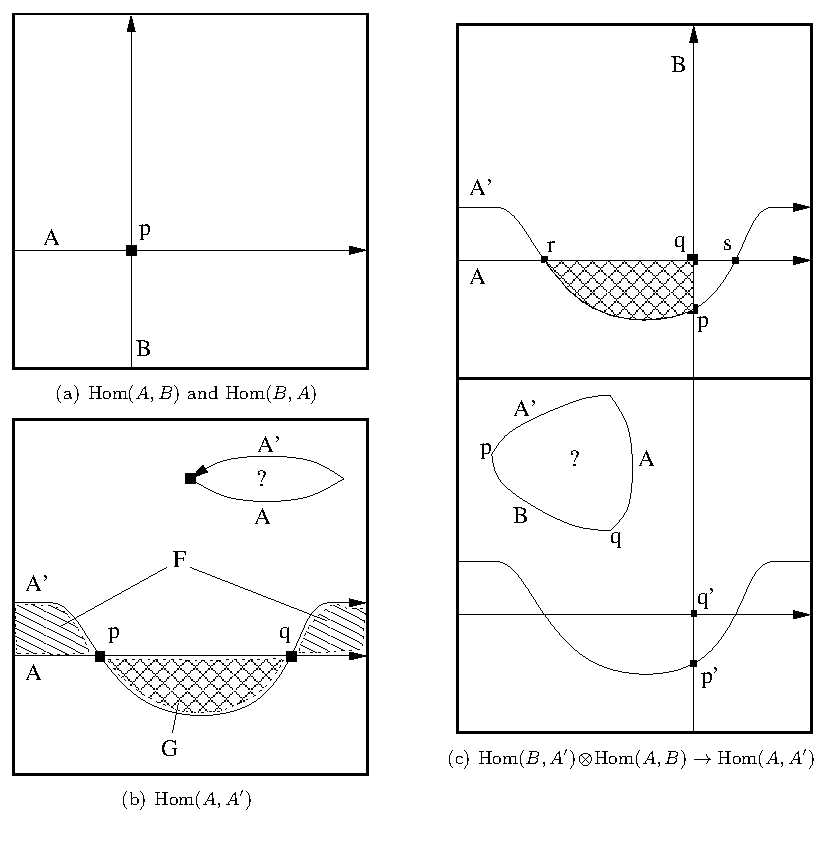
\includegraphics[width=0.92\textwidth]{figures/fig2.pdf}
  \caption{二维球面 $S^2$ 上闭曲线的同伦类。(左) 参数域 $(s,t)\in[0,1]^2$，边界整体映为基点 $r_0$，
           竖直箭头表示 $t$ 增大方向；(右) 球面 $\Sigma$ 上对应的闭曲线族，均自基点 $r_0$ 出发并回到 $r_0$。
           原文仅标 “Figure 2”（原文 PDF 第 15 页），无说明性图注。}
  \label{fig:2}
\end{figure}
% [Tutor Note: 图 2 的读法，见原文 PDF 第 15 页。$(s,t)$ 正方形的整个边界都映到基点 $r_0$，故对每个固定的 $s$，$t\in[0,1]$ 是 $\Sigma$ 上一条由 $r_0$ 出发又回到 $r_0$ 的闭曲线；右图中这些闭曲线按同伦类分层，其绕数即磁荷。注意左图中竖直箭头只表示 $t$ 增大方向，图中的“曲线族”是同一映射 $r(s,t)$ 在不同 $s$ 处的像。]

沿 $t$ 方向的协变导数为
$$
D_t \phi(s,t) =\frac{\partial r^i}{\partial t}D_i \phi(s,t)=0\,.
$$
对常数 $s$，可把它解出为
$$
\phi(s,t)=g(s,t)\phi(s,0)\,, 
$$
其中 $g(s,t)$ 满足 $D_t g=0$、$g(s,0)=1$，并由路径编序积分给出
\begin{equation}
g (s,t) =  P\left(\,\exp \left(\,ie\int^{t}_{0}
\vec{W}\cdot\frac{\partial \vec{r}}{\partial t} \, dt\right)\right)\,. 
\label{LVIII}
\end{equation}
% [Tutor Note: 见原文 PDF 第 15 页式 (36)。$P$ 表示路径编序（沿 $t$ 增大方向）；指数中 $ie\int\vec{W}\cdot d\vec{r}$ 的量纲须与式 (33) 的 $D_\mu=\partial_\mu+ieW_\mu$ 一致，核对时勿额外添加 $e$ 或 $2\pi$。]
显然，$g(s,t)$ 是 $G$ 的一个元素，它通过规范变换把任意 $\phi(s,t)$ 变到参考值 $\phi(s,0)$，而 $\phi(s,0)=\phi_0$ 与 $s$ 无关。因此，$g(s,t)$ 包含与 $\phi(s,t)$ 相同的拓扑信息，并由 $\pi_2(G/H)$ 中的一个同伦类刻画。由于在 $s=0,1$ 处 $\partial r/ \partial t =0$，故 $g(0,t)=g(1,t)=1$。当 $t=1$ 时，$\phi(s,1)=g(s,1)\phi_0$。但由于 $\phi(s,1)=\phi_0$，我们断定 $g(s,1)$ 必为未破缺规范群 $H$ 的元素，并把它记为 $h(s)$：
\begin{equation}
h(s)\equiv g(s,1)=P\,\exp\left(ie\int^1_0\,\vec{W}\cdot\frac{\partial
\vec{r}}{\partial t}\,dt\right)\,. 
\label{LIX}
\end{equation}
由于 $h(1)=h(0)=1$，当我们沿 $s$ 移动时，$h(s)$ 描述 $H$ 中的一条闭路径，因而属于 $\pi_1(H)$。然而要注意，当 $t$ 从 $1$ 变到 $0$ 时，$g(s,t)$ 在 $h(s)$ 与恒等元之间连续插值。因此，$h(s)$ 只能描述 $H$ 中那些在 $H$ 嵌入 $G$ 后同伦于平庸路径的闭路径。我们把 $\pi_1(H)$ 中对应于这类路径的子群记为 $\pi_1(H)_G$。若映射 $\phi(s,t)$ 的同伦类在 $\pi_2(G/H)$ 中改变，则 $h(s)$ 的同伦类在 $\pi_1(H)_G$ 中改变。事实上，$\pi_2(G/H)$ 与 $\pi_1(H)_G$ 之间存在一一对应，两个群同构 \cite{coleman1}。于是，我们同样可以用其在 $\pi_1(H)_G$ 中的同伦类来刻画磁单极。

让我们更详细地讨论这一点。由于 $H$ 中的任何闭路径也是 $G$ 中的闭路径，存在从 $\pi_1(H)$ 到 $\pi_1(G)$ 的自然同态。如上文讨论所示，$\pi_1(H)_G$ 位于该同态的核中。此外，对紧致连通群 $G$，$\pi_2(G)=0$，这意味着 $\pi_2(G)$ 可作为单位元嵌入 $\pi_2(G/H)$。我们上面所做的，基本上是构造了如下正合序列的一部分：
$$
\pi_2(G)\rightarrow\pi_2(G/H)\rightarrow\pi_1(H)\rightarrow 
\pi_1(G)\rightarrow\pi_1(G/H)\rightarrow\pi_0(H)
$$
% [Tutor Note: 含糊点拨，见原文 PDF 第 16 页的正合序列。原文“$\pi_2(G)$ 可作为单位元嵌入 $\pi_2(G/H)$”的措辞不严谨：对紧致连通 $G$ 有 $\pi_2(G)=0$，于是由正合性得 $\pi_2(G/H)$ 单射地映入 $\pi_1(H)$，其像正是（在 $G$ 中同伦于平庸路径的）$\pi_1(H)_G$，故 $\pi_2(G/H)\cong\pi_1(H)_G$。原文所谓“嵌入”只是说明 $\pi_2(G)=0$ 这一环在序列中不贡献，读者不必按字面理解为群嵌入。完整讨论见文献 [2]（Coleman）。]
注意若 $G$ 单连通，则 $\pi_1(G)=0$ 且 $\pi_1(H)_G=\pi_1(H)$，于是整个 $\pi_1(H)$ 都进入磁单极的物理描述。对非单连通的 $G$，这种情况可以在存在狄拉克弦时实现。这样的弦表现为 $(s,t)$ 平面上的一个奇点；在它存在时，不再能把 $h(s)$ 连续形变到恒等映射。因此 $h(s)$ 的同伦类不再受限于 $\pi_1(H)_G$。然而，对非单连通的 $G$，只要把 $G$ 嵌入其万有覆盖群 $\tilde G$，仍可用不受限制的 $\pi_1$ 群来描述。我们用 $\hat H$ 表示 $\phi$ 的小群。由于 $\tilde G$ 必定连通，$\pi_1(\tilde G)=0$ 且 $\pi_1(\hat H)= \pi_1(H)_G$。作为例子，考虑 Georgi–Glashow 模型。这里 $G = SO(3)$（其中 $(Ta)_{ij}=-i\epsilon_{aij}$），$\tilde{G} = SU(2)$（其中 $T_a=\frac{1}{2}\sigma_a$）。$H$（或 $\hat H$）中同伦不等价的路径为：
$$
h(t)=\exp(it\,\vec{\phi}\cdot\vec{T}\,4\pi N/a),\quad {\rm for}\,\,\, 
0 \leq t \leq 1\,.
$$
刻画 $\pi_1$ 中元素的整数 $N$ 如下确定：
$$
\begin{array}{llll}
\tilde G=SU(2),& \tilde H=U(1),& \vec{\phi}\cdot\vec{T}\in 
\frac{1}{2}{\bf Z},& \Rightarrow\,\, N \in {\bf Z}\,, \cr
G=SO(3),& H=SO(2),& \vec{\phi}\cdot\vec{T}\in {\bf Z},&
\Rightarrow\,\, N \in \frac{1}{2}{\bf Z}\,.
\end{array}
$$
由于 $SO(3)\sim S^2/{\bf Z}_2$，两种情形下都只有整数 $N$ 的路径有贡献。后面我们会证明 $g=4\pi N/e$。对 $SU(2)$，$q_0=e\hbar/2$ 且 $gq_0/4\pi\hbar=N/2$；对 $SO(3)$，$q_0=e\hbar$ 且 $gq_0/4\pi\hbar=N$。
% [Tutor Note: 见原文 PDF 第 16 页。原文称“后面我们会证明 $g=4\pi N/e$”，但本分片后文并未再给出独立证明；读者可对照式 (37)–(42) 的广义量子化条件自行补出（比较 $h(t)$ 的指数中 $4\pi N/a$ 的归一化与式 (41) 中 $G_0$ 前的 $ie/4\pi$）。另注意半整数 $N$ 的路径在 $SO(3)$ 中虽闭合，却生成 $\pi_1(SO(3))={\bf Z}_2$ 的非平凡类，不在 $\pi_1(H)_G$ 中，故最终两种情形都只保留整数 $N$。]

对 Glashow–Weinberg–Salam 模型，$G=SU(2)\times U(1)$，$H=U(1)$ 是 $SU(2)$ 与 $U(1)$ 的线性组合。虽然 $\pi_{1} (H) = {\bf Z}$，但 $\pi_{1} (H)_{G} = 0$。因此在该模型中，任何非平凡磁单极都必须带有狄拉克弦。

我们的目标是只用未破缺规范场（$H$ 场）来描述磁单极。虽然已经得到了用 $\pi_1(H)_G$ 的表述，但由 (\ref{LIX}) 给出的 $h(s)$ 只涉及 $H$ 场这一点并不显然。下面来说明：量 $g^{-1}(s,t)D_s g(s,t)$ 在依赖于 $t$ 的规范变换下不变。此外，由构造 $D_t g(s,t)=0$。因此可以写出
\begin{equation}
\partial_t(g^{-1}D_s g)= D_t(g^{-1}D_s g)=g^{-1}[D_t,D_s] g =
ie g^{-1} G_{ij} g \frac{\partial r^i}{\partial t} \frac{\partial r^j}
{\partial s}\,.
\label{LX}
\end{equation}
把上式的第一项与最后一项从 $t=0$ 积分到 $t=1$。由于 $t=0$ 时 $g^{-1}D_s g=0$、$t=1$ 时 $g^{-1}D_s g=h^{-1}dh/ds$，我们得到
\begin{equation}
h^{-1} \, \frac{dh}{ds} = ie \, \int^{1}_{0} dt \,
g^{-1} G_{ij}\,g \,\frac{\partial r^i}{\partial t} \,
\frac{\partial r^j}{\partial s}\,.
\label{LXI}
\end{equation}
由于 $G_{ij}$ 是在 $\Sigma$ 上计算的，它只涉及 $H$ 规范场。用 $g$ 作共轭不会引入对重规范场的依赖，这从方程的左边可以明显看出。因此映射完全由 $H$ 场给出，与希格斯场无关。作为一个简单应用，考虑狄拉克磁单极。把 (\ref{LXI}) 从 $s=0$ 积分到 $s=1$，得到 $h(1)=exp(ie\int {\vec B}\cdot{\vec ds})$。由于 $h(1)=1$，这给出狄拉克量子化条件 $eg=2\pi n$，或 $qg/4\pi\hbar=n/2$。(\ref{LXI}) 的另一个有趣推论是对夸克分数电荷的一种可能解释。我们将在下一节描述这一点。

\subsection{磁单极与分数电荷}

到目前为止，我们已经看到磁单极的存在如何使电荷以整数单位量子化。然而在物理世界中，我们还会遇到带分数电荷的夸克。下面我们将看到，磁单极的存在如何也能解释这些分数电荷 \cite{CO,GO}。

让我们把伴随希格斯场表示为 $\phi=\phi^a T^a$，其中 $T^a$ 是基本表示矩阵。此外，我们只考虑上一小节所述的曲面 $\Sigma$ 上的 $\phi$。当 $\phi$ 处于希格斯真空中时，生成元 $T^a$ 属于 $G$ 的未破缺子群 $H$，当且仅当 $[T^a,\phi]=0$。这意味着 $\phi$ 本身就是 $H$ 的一个生成元，并且与其他生成元对易。因此 $H$ 的李代数为 $L(H)=u(1)\oplus L(K)$ 的形式，我们取 $L(K)$ 与 $u(1)$ 正交：对 $K^a\in K$ 有 ${\rm Tr}(\phi K^a)=0$。局域地，$H$ 具有 $U(1)\times K$ 的结构，但这未必是整体结构。我们把 $K$ 称为色群，并把 $U(1)$ 认同为电磁相互作用对应的群。$H$ 中的规范场可分解为 $W^\mu=A^\mu\phi/a + X^\mu$，其中 ${\rm Tr}(\phi X^\mu)=0$。展开协变导数 $\partial_\mu+ ie W_\mu$，可以确定与 $A_\mu$ 耦合的电荷算符为 $Q=(e\hbar/a)\phi$。

由于 $h^{-1} dh/ds$ 是 $H$ 的一个生成元，我们可以写出
\begin{equation}
h^{-1} \frac{dh}{ds}=ie\alpha (s)\,\frac{\phi_0}{a} +
i \beta_{a} K^{a} \,.
\label{hab}
\end{equation}
利用 ${\rm Tr}(T_a T_b)=\delta_{ab}$、$\phi(r)=g\phi_0 g^{-1}$ 以及方程 (\ref{LXI})，得到
\begin{eqnarray}
\alpha (s)&=&-\frac{i}{ae}{\rm Tr}\left(\phi_0 h^{-1}\frac{dh}{ds} 
\right) \nonumber \\
&=&\frac{1}{a} \int^{1}_{0}{\rm Tr} \left(\varphi (r) G_{ij}\right) 
\frac{\partial r^i}{\partial t}\frac{\partial r^j}{\partial s}\,dt\,.
\nonumber
\end{eqnarray}
把电磁场强张量确定为 $F^{\mu\nu}={\rm Tr}\,(\phi G^{\mu\nu}/a)$，我们得到 $\alpha(s)= d\Omega/ds$，其中 $\Omega(s)$ 是固定 $s$ 时路径 $0\leq t\leq 1$ 在 $S^2$ 上于原点处所张立体角内的磁通量。把它代回 (\ref{hab}) 并从 $s=0$ 积分到 $s$，得到
$$
h(s)= k(s) e^{i Q \Omega(s) / \hbar}\,.
$$
% [Tutor Note: 含糊点拨，见原文 PDF 第 17 页。原文“the magnetic flux in a solid angle subtended at the origin by the path”措辞较绕：应理解成“穿过该路径所张立体角（以原点为顶点）的磁通量”，即 $\Omega(s)$ 本身是立体角、乘以 $B$ 才是通量；这正是 $\alpha(s)=d\Omega/ds$ 的几何含义。]
由于 $h(1)=1$ 且 $\Omega (1) = g$（其中 $g$ 是 $\Sigma$ 内部的总磁荷），量子化条件被替换为
$$
e^{igQ/\hbar} = k(1)^{-1}=k \in K \,.
$$
左端在 $K$ 下不变，因此我们最多只能有 $k\in {\bf Z}(K)$，即 $K$ 的中心。若取 $K = SU(N)$，则 $k=e^{2\pi in/N}$，其中 $n=1,2,\dots N$。如果所有 $n$ 值都被允许，则 $U(1)\cap K\subset Z_{N}$。这对应于整体上 $H$ 不能分解为 $U(1)\times K$ 这一事实。现在，设 $|s>$ 是一个色单态。则 $k|s> = |s>$ 且 $exp(igq_s/\hbar)=1$，这又是狄拉克量子化条件。于是，若 $q_0$ 与 $g_0$ 是色单态的电荷与磁荷单位，则 $q_s=n_sq_0$，$g=mg_0$，且 $g_0q_0=2\pi\hbar$。色非单态 $|c>$ 可按其在色群 $K$ 的中心下的行为分类：
$$
k|c> = e^{2\pi i \, t(c)/N} |c> =e^{igQ / \hbar} |c>\,,
$$
其中 $t(c)$ 是模 $N$ 的整数。对最小磁单极 $g_{0}$，我们得到 $g_0 q_c /\hbar=2\pi(m + t(c)/N) $，因此
$$
q_c = q_0 (m + \frac{t(c)}{N})\,. 
$$
若像 QCD 那样取 $N=3$ 且 $m=0$，则 $q_c=q_0/3, 2q_0/3,q_0$。
% [Tutor Note: 含糊点拨，见原文 PDF 第 18 页。原文“If all values of $n$ are allowed, then $U(1)\cap K\subset Z_N$”一步较绕：其含义是整体上 $H$ 不是直积 $U(1)\times K$，而是 $(U(1)\times K)/Z_N$ 型的结构，故 $U(1)$ 与 $K$ 的中心在整体上重合；对色单态（$k=1$）回到通常的狄拉克条件，而对色非单态则得到以 $1/N$ 为单位的分数电荷。注意原文用 $|s>$、$|c>$ 而不是 $|s\rangle$、$|c\rangle$，系作者笔误，译文照录。]

\subsection{非阿贝尔磁荷与 Montonen–Olive 猜想}

本小节我们首先考虑把电荷量子化推广到非阿贝尔磁单极 \cite{GNO}，然后描述 Montonen 与 Olive 的电磁对偶猜想 \cite{MO}。

Goddard、Nuyts 与 Olive \cite{GNO} 试图对所有 $H$-磁单极位形进行分类。为描述这样的磁单极，我们考虑静态位形并取规范 $\vec{r}\cdot\vec{W}^a =0$。在大距离下，可合理地把场强的磁场分量写成
$$
G_{ij} = \frac{1}{4 \pi r^2} \, \epsilon_{ijk} \, \hat{r}^k G(r)\,, 
$$
其中 $D_\mu G(r)=0$。由于 $G(r)$ 按伴随表示变换，可以写成 $G(r)=g(s,t)G_{0}g(s,t)^{-1}$。把上述表达式代入 (\ref{LXI}) 并对 $s$ 积分，得到
\begin{eqnarray}
{\rm ln}\left(h(s)\right) & = & \frac{ie}{4\pi r^2} G_0  
\int^s_0 ds\int^1_0 dt\,\epsilon_{ijk}\hat{r}^k \,
\frac{\partial r^i}{\partial t}\frac{\partial r^j}{\partial s}
\nonumber \\
& = & \frac{ie}{4\pi} G_0\,\Omega (s)\,.
\label{LXX}
\end{eqnarray}
% [Tutor Note: 原文笔误，见原文 PDF 第 18 页：“the magnetic componenets”中 “componenets” 应为 “components”。]
这里 $\Omega (s)$ 是 $S^2$ 上环路 $0\leq t\leq 1,\,s={\rm const}$ 在原点张开的立体角。于是 $\pi_1(H)_G$ 中的元素为
$$
h(s)= e^{\frac{ie}{4 \pi} G_0\Omega(s)}\,. 
$$
由于 $h(1)=1$，上式意味着
\begin{equation}
e^{ie G_0} = 1\,,
\label{LXXI} 
\end{equation}
这就是广义的电荷量子化条件。显然，$G_0$ 在规范群中的共轭变换下是任意的。这一自由度可用来求解电荷量子化条件，如下所述：假定 $H$ 紧致且连通，令 $T$ 表示由 $H$ 的嘉当子代数生成的阿贝尔子群。那么 $H$ 的任一元素都至少与 $T$ 的一个元素共轭。因此总能找到某个标架使 $G_0 = \beta^a T^a$。系数 $\beta^a$ 仍不唯一，因为它们在保持 $G_0$ 这一参数化不变的 $H$ 外尔群下变换。因此，由外尔群作用相联系的 $\beta^a$ 的等价类，才是刻画非阿贝尔磁荷的规范不变对象。$\beta^a$ 由量子化条件 $exp(ie \beta^a T^a)=1$ 决定。为解出它，令 $\omega^a$ 表示 $H$ 在给定表示中的权矢量，$\Lambda(H)$ 表示权格。则量子化条件意味着
$$
e \beta^a \omega^a \in 2\pi{\bf Z}\,,\qquad {\rm for\, all}\,\, 
\omega\in \Lambda(H)\,.
$$      
注意 $e$ 与 $2\pi$ 的因子依赖于约定。因此 $e\beta$ 位于与 $\Lambda(H)$ 对偶的格上：$e\beta \in \Lambda^*(H)$。这个对偶格本身可视为某个对偶群 $H^v$ 的权格，它以 $e\beta$ 为权矢量（详见 \cite{GNO}）。此外，$(H^v)^v=H$。$H$ 称为电群，$H^v$ 称为磁群。磁荷与 $H^v$ 的关系，和电荷与 $H$ 的关系完全相同。对偶群对的一个简单例子由 $SO(3)$ 与 $SU(2)$ 提供。此时 $G_0=\beta T^3$。$T^3$ 对 $SO(3)$ 有整本征值，对 $SU(2)$ 有半整本征值。量子化条件 $exp(ie\beta T^3)=1$ 给出：
% [Tutor Note: 见原文 PDF 第 18–19 页。由式 (42) 得到 $e\beta^a\omega^a\in2\pi{\bf Z}$ 后，$e\beta$ 落在与权格 $\Lambda(H)$ 对偶的格 $\Lambda^*(H)$ 上；原文随即把这个对偶格解释为对偶群 $H^v$ 的权格。这一步依赖 $H$ 的表示与归一化约定（原文也明说 “factors of $e$ and $2\pi$ are convention dependent”），下面 $SO(3)$ 与 $SU(2)$ 的例子正是用 $T^3$ 的整/半整本征值来体现这种约定依赖。]
\begin{eqnarray}
{\rm for}\,\,\,H=SO(3)\,:\quad e\beta &=& 4\pi \frac{n}{2}=4\pi \times 
({\rm weight \,\,of\,\,} SU(2))\,, \nonumber\\ 
{\rm for}\,\,\,H=SU(2)\,:\quad e\beta &=& 4\pi n = 4\pi \times 
({\rm weight\,\,of\,\,}SO(3))\,. \nonumber
\end{eqnarray}
对一般的 $SU(N)$ 群，对偶关系为 $(SU(NM)/{\bf Z}_N)^v = (SU(NM)/{\bf Z}_M)$，特别地，$SU(N)^v = SU(N)/Z_N$。

现在，我们简要描述以上述结果为基础的 Montonen–Olive 猜想 \cite{MO}。该猜想断言：一个规范理论由 $H \times H^{v}$ 刻画，并且该理论有两种等价的描述：一种用 $H$ 规范场，其微扰谱中是通常的带电粒子；另一种用 $H^{v}$ 规范场，其微扰谱中是磁单极。与电荷相联系的 Noether 流，同样与和磁荷相联系的拓扑流互换。因此，$H$ 理论的耦合常数 $q/\hbar$ 在对偶的 $H^v$ 理论中由 $g/\hbar$ 替代。由于 $g\sim 1/e$，该猜想把一个强耦合理论与一个弱耦合理论联系起来，反之亦然。因此，要证明或否证这个猜想都不容易。Montonen 与 Olive 在 Georgi–Glashow 模型的 BPS 极限下给出了支持该猜想的一些半经典证据。该模型的微扰谱包含一个希格斯玻色子、一个光子与两个有质量的带电矢量玻色子，另以磁单极作为孤子型经典解。未破缺的规范群是自对偶的，$H=U(1)=H^v$，因此对偶理论与原理论形式相同，只是磁单极成为基本态，而有质量的规范玻色子成为孤子解。对偶理论中规范玻色子的质量（在那里它以孤子出现）可用 BPS 公式计算，结果正好是正确值。此外，Manton \cite{manton} 得到的两磁单极之间的长程力，也可通过计算对偶理论中 $W$ 玻色子之间的势得到，结果相同。
% [Tutor Note: 原文笔误，见原文 PDF 第 19 页。本页有三处拼写错误：“weekly coupled”应为“weakly coupled”，“monoples”应为“monopoles”，“superysymmetry”应为“supersymmetry”；另有“in the in the $H^v$-theory”重复了“in the”（在原文 PDF 第 19 页下半页）。物理上注意：Montonen–Olive 猜想交换的是微扰谱中的基本粒子与孤子，即 $H$ 理论与 $H^v$ 理论互换，耦合常数 $q/\hbar\leftrightarrow g/\hbar$；在自对偶的 $H=U(1)=H^v$ 情形，这一互换表现为 $e\leftrightarrow g=4\pi/e$，即强耦合与弱耦合互换。]

由于 Montonen–Olive 对偶本质上是非微扰的，除非我们对理论的微扰与非微扰方面有某种控制，否则无法在微扰框架内验证它。超对称恰恰提供了这种控制。事实上，在 $N=4$ 超杨–米尔斯理论中，该对偶的一些非常非平凡的预言已在 \cite{sen} 中得到验证。在后面的部分中，我们将详细讨论 $N=2$ 超对称规范理论中 Montonen–Olive 对偶的类比。然而，其先决条件是在杨–米尔斯作用量中引入 $\theta$ 项，它会改变双子的电荷。

\subsection{$\theta$ 参数与磁单极电荷}

本节中我们将遵循 Witten \cite{Witten79} 证明：当拉格朗日量中存在 $\theta$ 项时，粒子的磁荷总会对其电荷有贡献。

如 Schwinger 与 Zwanziger 所证明，对电荷为 $(q_1,g_1)$ 与 $(q_2,g_2)$ 的两个双子，量子化条件取形式
\begin{equation}
q_1g_2 - q_2g_1 = 2 \pi n \hbar
\label{LXXVI}
\end{equation}
对一个电荷 $q_0$ 与一个双子 $(q_n,g_n)$，这给出 $q_0g_n = 2\pi n\hbar$。因此双子可能具有的最小磁荷为 $g_0=2\pi\hbar/q_0$。对两个具有相同磁荷 $g_0$、电荷分别为 $q_1$ 与 $q_2$ 的双子，量子化条件意味着 $q_1-q_2= nq_0$。因此，虽然电荷之差是量子化的，单个电荷仍可任意。双子电荷的这种任意性在理论 CP 不变时可如下确定：在 CP 变换下 $(q,g)\rightarrow (-q,g)$。若理论 CP 不变，态 $(q,g_0)$ 的存在必然导致 $(-q,g_0)$ 的存在。把量子化条件用于这一对态，得到 $2q =q_0\times integer$。这意味着 $q=nq_0$ 或 $q=(n+\frac{1}{2})q_0$，不过在同一个理论中只能出现整数电荷或半奇数电荷的双子，而不能两者兼有。

在上述论证中，为得到双子电荷的整数或半奇数整数值，假定 CP 不变是关键的。然而在现实世界中 CP 不变性被破坏，没有理由期待电荷按上述方式量子化。为研究 CP 破坏的效应，我们考虑在 Georgi–Glashow 模型中加入一个 $\theta$ 项，它是 CP 破坏的来源：
% [Tutor Note: 原文笔误，见原文 PDF 第 20 页：“half-odd inegral values”中 “inegral” 应为 “integral”；译文按正确含义处理。]
\begin{equation}
{\cal L}=-\frac{1}{4}\,F^a_{\mu\nu}F^{a\mu\nu}+\frac{1}{2}
(D_{\mu} \vec{\phi})^{2} - \lambda (\phi^{2} - a^{2} )^{2}
+\frac{\theta e^2}{32\pi^2}\,F^a_{\mu\nu}\tilde F^{a\mu\nu}\,. 
\label{LXXVIII}
\end{equation}
这里 $\tilde F^{a\mu\nu}=\frac{1}{2}\epsilon^{\mu\nu\rho\sigma} F^a_{\rho\sigma}$，矢量记号用于表示规范空间中的指标。$\theta$ 项的存在不影响运动方程，但会改变物理，因为理论不再 CP 不变。我们想构造该理论中的电荷算符。理论具有 $SO(3)$ 规范对称性，但电荷与一个保持希格斯真空不变的未破缺 $U(1)$ 相联系。因此，我们定义一个算符 $N$，它实现绕 $\hat{\phi}$ 方向、规范参数为 $\Lambda^a = \phi^a/a$ 的规范转动。这些变换对应于电荷。在 $N$ 作用下，矢量 $\vec v $ 与规范场 $\vec A_\mu$ 变换为
$$
\delta \vec{v} = \frac{1}{a} \, \vec{\phi} \times \vec{v}\,, \quad
\delta \vec{A}_{\mu} = \frac{1}{ea} \, D_{\mu} \vec{\phi}\,.
$$
% [Tutor Note: 易错预警，见原文 PDF 第 20–21 页。核对 $\theta$ 项的归一化：$F^a_{\mu\nu}\tilde F^{a\mu\nu}$ 是全导数，$\partial_\mu K^\mu=\frac12\epsilon^{\mu\nu\rho\sigma}F^a_{\mu\nu}F^a_{\rho\sigma}$，故式 (44) 中系数取 $\theta e^2/32\pi^2$ 才能保证 $\theta\to\theta+2\pi$ 是物理上等价的周期；若把 $\tilde F$ 的 $\frac12$ 漏掉，$\theta$ 的周期会差一个因子 2。]
显然 $\vec{\phi}$ 保持不变。在大距离处 $|\phi|=a$，算符 $e^{2\pi i N}$ 是绕 $\hat{\phi}$ 的 $2 \pi$ 转动，因此 $\exp\,(2\pi iN)=1$。在其他地方，转角为 $2\pi |\phi|/a$。然而，由高斯定律，若规范变换在 $\infty$ 处为 $1$，它使物理态保持不变。因此只有变换的大距离行为才是重要的，$N$ 的本征值以整数单位量子化。现在用 Noether 公式计算 $N$：
$$
N=\int\,d^3x\left(\frac{\delta{\cal L}}{\delta\partial_0 A^a_i}\;
\delta A_{i}^{a} + \frac{\delta {\cal L}}{\delta \partial_{0}
\phi^{a}} \; \delta \phi^{a} \right )\,.
$$
由于 $\delta \vec\phi= 0$，只有规范部分（其中也包括 $\theta$ 项）有贡献：
\begin{eqnarray}
\frac{\delta}{\delta \partial_{0}A^{a}_{i}} \,
\left ( F^{a}_{\mu \nu} F^{a\mu\nu}\right) &=&
4F^{aoi} = -4 {\cal E}^{ai}\,, \nonumber\\
\frac{\delta}{\delta \partial_{0}A^{a}_{i}} \,
\left(\tilde{F}^a_{\mu\nu}F^{a\mu\nu}\right) &=&
2\epsilon^{ijk}F^a_{jk} =-4 {\cal B}^{ai}\,. \nonumber
\end{eqnarray}
于是得到
\begin{eqnarray}
N &=&\frac{1}{ae} \int d^{3}x D_{i}\vec{\phi} \cdot \vec{\cal E}^i
- \frac{\theta e}{8\pi^{2}a}\,\int d^3x \, D_{i}\vec{\phi}
\cdot \vec{\cal B}^i \nonumber\\
&=& \frac{1}{e} Q - \frac{\theta e}{8 \pi^2} M \,,\nonumber
\end{eqnarray}
其中我们用了方程 (\ref{gq})。这里 $Q$ 与 $M$ 是电荷与磁荷算符，本征值分别为 $q$ 与 $g$，而 $N$ 以整数单位量子化。由此得到电荷的如下公式
$$
q=ne + \frac{\theta e^2}{8\pi^2} g \,.
$$  
% [Tutor Note: 原文笔误，见原文 PDF 第 21 页：“with eigenvalues $q$ and $g$, respectivly”中 “respectivly” 应为 “respectively”。另，这里的 $n$ 是 $N$ 的本征值（整数），与 §1.9 中刻画 $\pi_1$ 的整数 $N$ 无关。]
对 't Hooft–Polyakov 磁单极，$n=1$，$g=-4\pi/e$，因此 $q=e(1-\theta/2\pi)$。对一般的双子解，我们得到
\begin{equation}
g= \frac{4\pi}{e} m,\qquad q = ne + \frac{\theta e}{2\pi}m\,.
\label{gqtheta}
\end{equation}
% [Tutor Note: 易错预警，见原文 PDF 第 21 页式 (45)。这里 $g=\frac{4\pi}{e}m$ 的 $m$ 与电荷公式中 $ne$ 的 $n$ 是彼此独立的整数。对 't Hooft–Polyakov 单极，$g=-4\pi/e$ 意味着 $m=-1$（原文只写了“$n=1$”），代回式 (45) 才得到 $q=e(1-\theta/2\pi)$；若误取 $m=1$，会得到 $q=e(1+\theta/2\pi)$。]
因此，在存在 $\theta$ 项时，磁单极总是带有电荷，而该电荷不是某个基本单位的整数倍。

把带电态表示为复平面上的点非常有用：电荷沿实轴，磁荷沿虚轴。于是，一个态可表示为
\begin{equation}
q+ig=e(n+m\tau)\,,
\label{qig}
\end{equation}
其中
\begin{equation}
\tau=\frac{\theta}{2\pi} + \frac{4\pi i}{e^2}
\label{tau}
\end{equation}
在此参数化下，Bogomol'nyi 界 (\ref{Bbound}) 取形式
\begin{equation}
M \geq {\sqrt 2}|ae(n+m\tau)|\,.
\label{BBtau}
\end{equation}
注意 (\ref{qig}) 意味着所有态都位于一个格参数为 $\tau$ 的二维格点上，而 (\ref{BBtau}) 意味着一个态的 BPS 界正比于其格点到原点的距离。这些方程在后续讨论中起着非常重要的作用。
% [Tutor Note: 见原文 PDF 第 22 页式 (46)–(48)。$\tau=\theta/2\pi+4\pi i/e^2$ 的实部为 $\theta/2\pi$、虚部为 $4\pi/e^2$；式 (48) 的 BPS 界即“质量不小于其格点到原点距离”，这正是后文（§2 起）把 BPS 态、格点与单值变换联系起来的出发点，建议牢记式 (46)–(48) 这三个式子。]
